\section{Appendix}
\label{sxn:appendix}

In this appendix, we provide more details on several issues that are important for reproducibility of our results.

\subsection{Reproducibility Considerations}


\paragraph{SVD of Convolutional 2D Layers.}

There is some ambiguity in performing spectral analysis on Conv2D layers.  
Each layer is a 4-index tensor of dimension $(w,h,in,out)$, with an $(w\times h)$ filter (or kernel) and $(in, out)$
channels. When $w=h=k$,  giving $(k\times k)$ tensor slices, or \emph{pre-Activation Maps} $\mathbf{W}_{i,L}$ of dimension $(in\times out)$ each. 
%
We identify 3 different approaches for running SVD on a Conv2D layer:
\begin{enumerate}
\item run SVD on each pre-Activation Map $\mathbf{W}_{i,L}$, yielding $(k\times k)$ sets of $M$ singular values
\item stack the maps into a single matrix of, say, dimension $((k\times k\times out)\times in)$, run SVD to get $in$ singular values
\item compute the 2D Fourier Transform (FFT) for each of the $(in, out)$ pairs, and run SVD on the Fourier coeffients~\cite{CNNSVD}, leading to $\sim(k\times in\times out)$ non-zero singular values.
\end{enumerate}
Each method has tradeoffs.  
Method (3) is mathematically sound, but computationally expensive. Method (2) is ambiguous.
For our analysis, because we need thousands of runs, we select method (1), which is the fastest (and is easiest to reproduce).

\paragraph{Normalization of Empirical Matrices.}  
Normalization is an important, if underappreciated, practical issue.
Importantly, the normalization of weight matrices does \emph{not} affect the PL fits because $\alpha$ is scale-invariant.
Norm-based metrics, however, do depend strongly on the scale of the weight matrix--that is the point.
%\nred{Indeed, early theoretical work by Bartlett suggests that the test accuracy depends strongly on the ``total size'' of the weight matrics.}
To apply RMT, we usually define $\mathbf{X}$ with $1/N$ normalization, assuming variance of $\sigma^{2}=1.0$.
%\footnote{For Heavy Tailed theorems, one typically needs a normalization such as \nred{$1/N^{\alpha-1}$. check this}}
Pretrained DNNs are typically initialized with random weight matrices $\mathbf{W}_{0}$, with
 $\sigma^{2}\sim 1/\sqrt{N}$, or some variant, e.g., the Glorot/Xavier normalization~\cite{GloBen10}, or a $\sqrt{2/Nk^2}$ normalization for Convolutional 2D Layers. With this implicit scale, 
we do \emph{not} ``renormalize'' the empirical weight matrices, i.e., we use them as-is.
The only exception is that \emph{we do rescale} the Conv2D pre-activation maps $\mathbf{W}_{i,L}$ 
by $k/\sqrt{2}$ so that they are on the same scale as the Linear / Fully Connected (FC) layers.

\paragraph{Special consideration for NLP models.}
NLP models, and other models with large initial embeddings require special care because the
embedding layers frequently lack the implicit $\frac{1}{\sqrt{N}}$ normalization present in other layers.
For example, in GPT, most layers, the maximum eigenvalue $\lambda_{max}\sim\mathcal{O}(10-100)$,
but in the first embedding layer, the maximum is of order N (the number of words in the embedding), or
 $\lambda_{max}\sim\mathcal{O}(10^{5})$.  For GPT and GPT2, we treat all layers as-is (although one may to normalize
the first 2 layers by  $\mathbf{X}$ by $\frac{1}{N}$, or to treat them as an outlier).

\subsection{Reproducing Sections 4 and 5}

We provide a github repository for this paper that includes Jupyter notebooks that fully reproduce all results.
All results have been produced using the weightwatcher tool (v0.2.7).
The ImageNet and OpenAI GPT pretrained models are provided in the current 
pyTorch~\cite{pytorch} and huggingface~\cite{higgingface} distributions, as specified in the \texttt{requirements.txt} file. 

\begin{table}[t]
\small
\begin{center}
\begin{tabular}{|p{1in}|c|}
\hline
Figure & Jupyter Notebook \\
\hline
1  &  WeightWatcher-VGG.ipynb \\
2(a)  &  WeightWatcher-ResNet.ipynb \\
2(b)  &  WeightWatcher-ResNet-1K.ipynb \\
3(a)  &  WeightWatcher-VGG.ipynb \\
3(b)  &  WeightWatcher-ResNet.ipynb \\
3(c)  &  WeightWatcher-DenseNet.ipynb \\
\hline
4 & WeightWatcher-Intel-Distiller-ResNet20.ipynb \\
\hline
5 & WeightWatcher-OpenAI-GPT.ipynb \\
6, 7 & WeightWatcher-OpenAI-GPT2.ipynb \\
\hline
\end{tabular}
\end{center}
\caption{Jupyter notebooks used to reproduce all results in sections ~\ref{sxn:cv} and ~\ref{sxn:nlp}}
\label{table:notebooks}
\end{table}

\subsection{Reproducing Figure~\ref{fig:resnet204D5L}, Distiller Model}

We provide the orginal Jupyter Notebooks, which uses the Intel \texttt{distiller} framework
.\footnote{\url{https://nervanasystems.github.io/distiller}} in the \texttt{distiller} folder of our 
github repo. Figure ~\ref{fig:resnet204D5L} is from the  \texttt{``...-Distiller-ResNet20.ipynb''} 
notebook (see Table~\ref{table:notebooks}).  
For completeness, we provide both the results described here, and additional results
on other pretrained and distilled models using the \texttt{weightwatcher} tool.

\subsection{Reproducing Table~\ref{table:results}, Section~\ref{sxn:all_cv_models} }

We provide several Google Colab notebooks which can be used to reproduce the of Section~\ref{sxn:all_cv_models}.
in the \texttt{ww-colab} folder in our github repo.  
The ImageNet-1K and other pretrained models are taken from the pytorch models in the \texttt{omsr/imgclsmob} 
``Sandbox for training convolutional networks for computer vision'' github repository~\cite{osmr}
The data for each regression can be generated in parallel by running each Google Colab notebook (i.e. \texttt{ww\_kdd2020\_0\_100.ipynb}) 
simultaneously on the same account.
The data generated is analyzed by the \texttt{ww\_kdd2020\_results.ipynb} notebook,
which runs all regressions and tabulates the results presented in Table~\ref{table:results}.

We attempt to run linear regressions for all pyTorch models for each architecture series for all datasets provided.  
There are over $450$ models in all, and we note that the \texttt{osmr/imgclsmob} repository is constantly being updated with new models.
We omit the results for CUB-200-2011, Pascal-VOC2012, ADE20K, and COCO datasets as there are less than 15 models
for those datasets.  And we filter out regressions with less than five datapoints.
The final datasets used are shown in Table~\ref{table:datasets}.
The final architecture series used are shown in  Table~\ref{table:architectures}, with the number of models in each.

To further explain how to reproduce our analysis, we run three batches of linear regressions. First at the global level, we divide models by datasets and run regression separately on all models of a certain dataset, regardless of the architecture. At this level, the plots are quite noisy and clustered as each architecture has its own accuracy trend but, you could still see that most plots show positive relationship with positive coefficients. The regressions are shown in Figure~\ref{fig:DSalphas}, as available in the results notebook.

To generate the results in Table 3, we run linear for each architecture series in Table~\ref{table:architectures},
regressing each empirical log norm metric against the reported Top 1 (and Top 5) errors (as listed on the \texttt{osmr/imgclsmob} github 
repository README file~\cite{osmr}, with the relevant data extracted and provided in our github repo as \texttt{pytorchcv.html}
We record the R-squared and mean squared errors (MSE) for each norm metric, averaged over all regressions for all architectures and datasets.
Plots are provided for every regression, and more fine grained results may be computed by the reader by 
analyzing the data in the \texttt{df\_all.xlsx} file.

\begin{table}[t]
\small
\begin{center}
\begin{tabular}{|p{1in}|c|}
\hline
Dataset & $\#$ of Models \\
\hline
imagenet-1k   &  78 \\
svhn          &  30 \\
cifar-100     &  30 \\
cifar-10      &  18 \\
cub-200-2011  &  12 \\
\hline
\end{tabular}
\end{center}
\caption{Datasets used}
\label{table:datasets}
\end{table}

\begin{table}[t]
\small
\begin{center}
\begin{tabular}{|p{2in}|c|}
\hline
Architecture & $\#$ of Models \\
\hline
ResNet                                     & 30 \\
SENet/SE-ResNet/SE-PreResNet/SE-ResNeXt    & 24 \\
DIA-ResNet/DIA-PreResNet                   & 18 \\
ResNeXt                                    & 12 \\
WRN                                        & 12 \\
DLA                                        & 6 \\
PreResNet                                  & 6 \\
ProxylessNAS                               & 6 \\
VGG/BN-VGG                                 & 6 \\
IGCV3                                      & 6 \\
EfficientNet                               & 6 \\
SqueezeNext/SqNxt                          & 6 \\
ShuffleNet                                 & 6 \\
DRN-C/DRN-D                                & 6 \\
ESPNetv2                                   & 6 \\
HRNet                      z                & 6 \\
SqueezeNet/SqueezeResNet                   & 6 \\
\hline
\end{tabular}
\end{center}
\caption{Architectures used}
\label{table:architectures}
\end{table}


\begin{figure}[t]
    \centering
    \subfigure[ImageNet 1K]{
        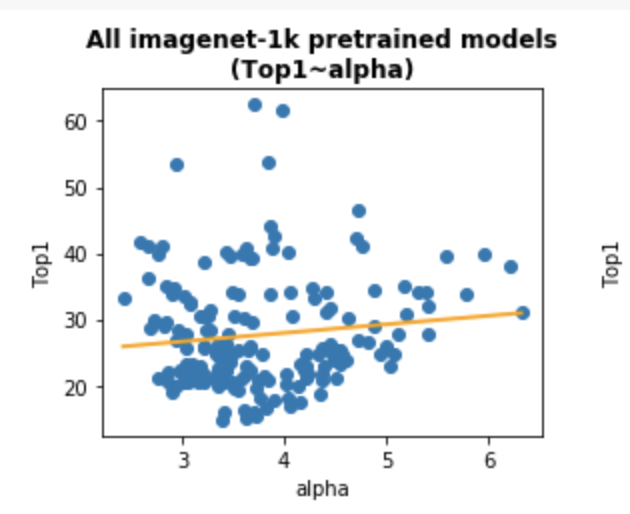
\includegraphics[width=2.5cm]{img/imagenet1k_alpha.png}
        \label{fig:imagenet1k-alpha}
    }
    \qquad
    \subfigure[ CIFAR 10 ]{
        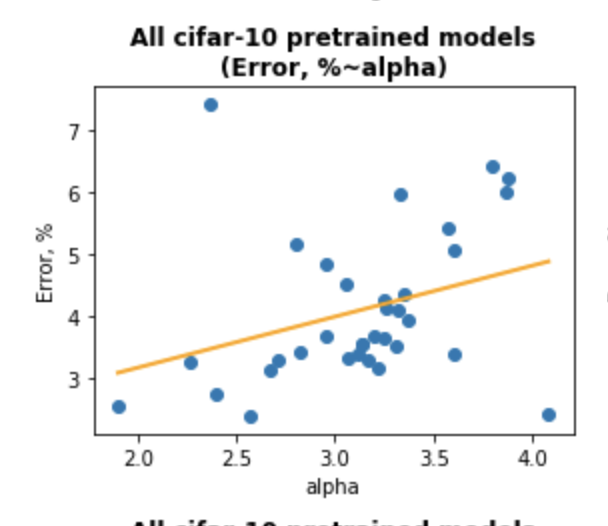
\includegraphics[width=2.5cm]{img/cifar10_alpha.png}
        \label{fig:cifar10.alpha}
    }
    \qquad
    \subfigure[ CIFAR 100 ]{
        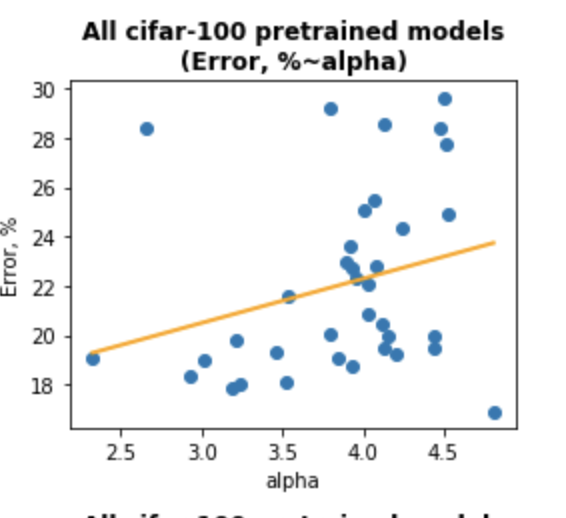
\includegraphics[width=2.5cm]{img/cifar100_alpha.png}
        \label{fig:cifar100.alpha}
    }
    \qquad
    \subfigure[ SVHN ]{
        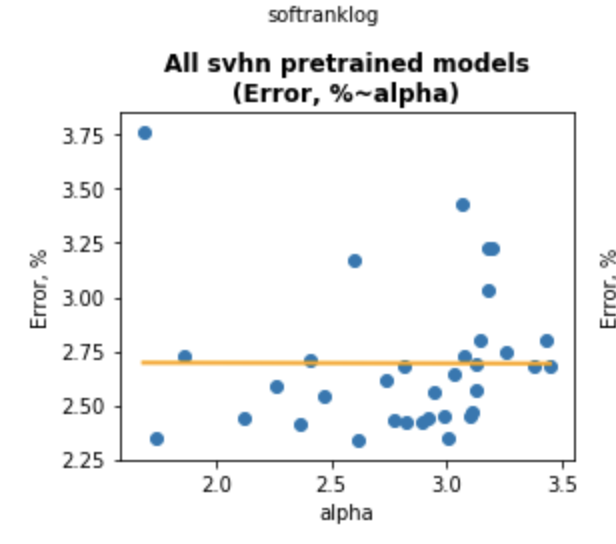
\includegraphics[width=2.5cm]{img/svhn_alpha.png}
        \label{fig:svhn.alpha}
    }
    \qquad
    \subfigure[ CUB 200 ]{
        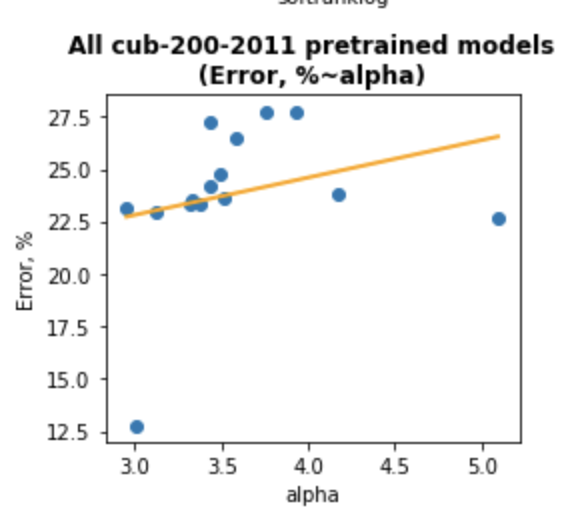
\includegraphics[width=2.5cm]{img/cub200_alpha.png}
        \label{fig:cub200.alpha}
    }
    \caption{\charles{Preliminary charts:} PL exponent $\alpha$ vs. reported Top1 Test Accuracies for pretrained DNNs available\charles{ref} for 5 different data sets.}

    \label{fig:DSalphas}
\end{figure}

 
